\subsection{Python Implementation}
	All code can be found at: \\ \href{https://github.com/Anonymous-Stranger/fft-image-encoding}{https://github.com/Anonymous-Stranger/fft-image-encoding}
	\subsubsection{DFT}
		See \ref{naive_dft_python} for our python implementation of the DFT. Our implementation of DFT doesn't use the matrix form of the equation. It uses two nested for loops, one to iterate over all $X_k$, and another to implement the summation over all $x_n$, using the standard formula. The inverse DFT is implemented in terms of the DFT, by reversing all but the first element of the input, computing the DFT and dividing all elements by the size of the input. The 2D DFT is implemented as two separate DFTs, one over the rows, and the other over the columns. It does this by taking the DFT over the rows, transposing the matrix, doing the DFT over the rows of the result (stored in a temporary), and then returning the transpose of the result. Both the inverse and 2D discrete fourier transform implementations take a function as input. This allowed us to use one function to implement it for both the naive DFT and Cooley-Tukey.
	\subsubsection{FFT}
		See \ref{cooley_tukey_python} for our python implementation of the FFT. Our implementation of Cooley-Tukey uses the simplest version, which only works on sets of data with a power of 2 size. It takes the input as a numpy array of complex values, uses python slicing to split into even and odd parts, recursively calling itself on each half (returning immediately when the size was 1), multiplying the odd values by the twiddle factors, and then concatenating the sum and difference of the even and odd values. The inverse and 2D discrete fourier transforms are implemented as described above.
\subsection{Results}
	\subsubsection{Performance}
		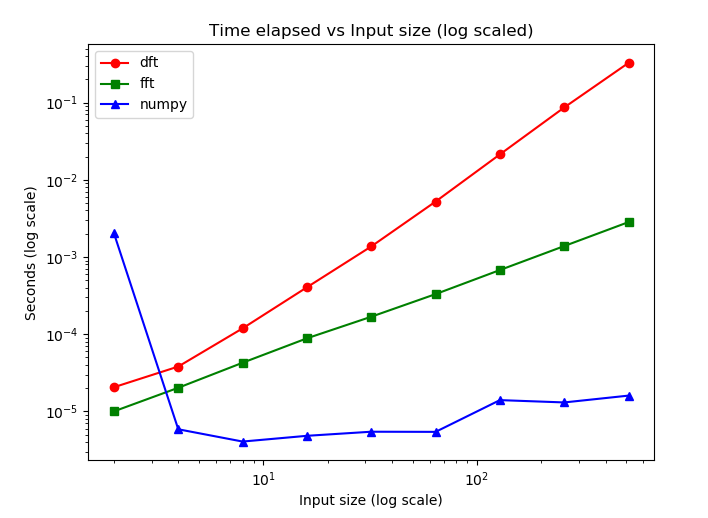
\includegraphics[width=\linewidth]{images/perfGraph.png}
		The graph above shows the performance of 3 different implementations of the discrete fourier transform on several different size inputs. The red line shows the time taken by the dft algorithm, the green line shows the time taken by our implementation of Cooley-Tukey, and the blue line shows the time taken by a library implementation. Because the distance between the red and green lines grows (on a log scale), it is easy to see that the naive algorithm is asymptotically slower than Cooley-Tukey. Aside from the anomaly at the first point, the reason the blue line looks as it does is because the library implements the algorithm in C, which is far faster than Python. As a result of this, not enough data points were tested for the algorithm to display its asymptotic behavior.
	\subsubsection{Compression}
		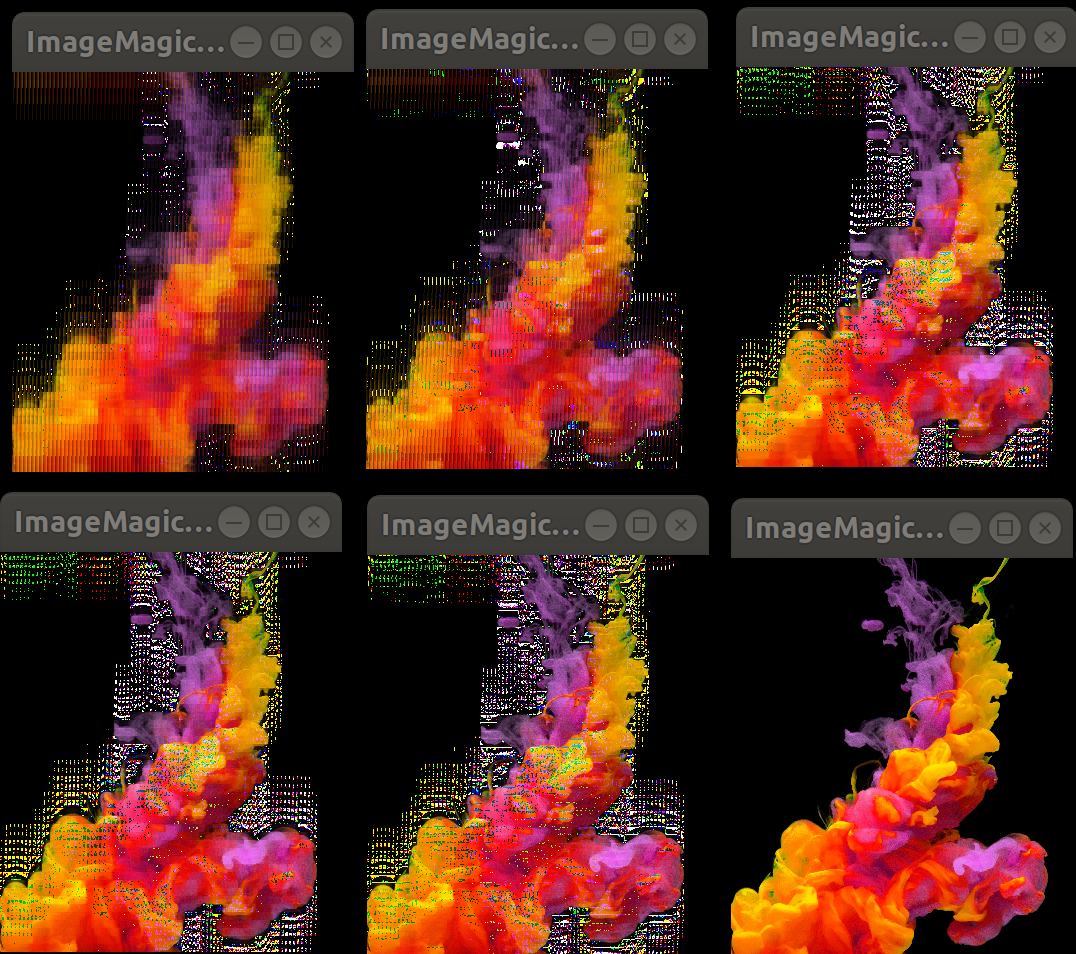
\includegraphics[width=\linewidth]{images/imgCompare1.png}
		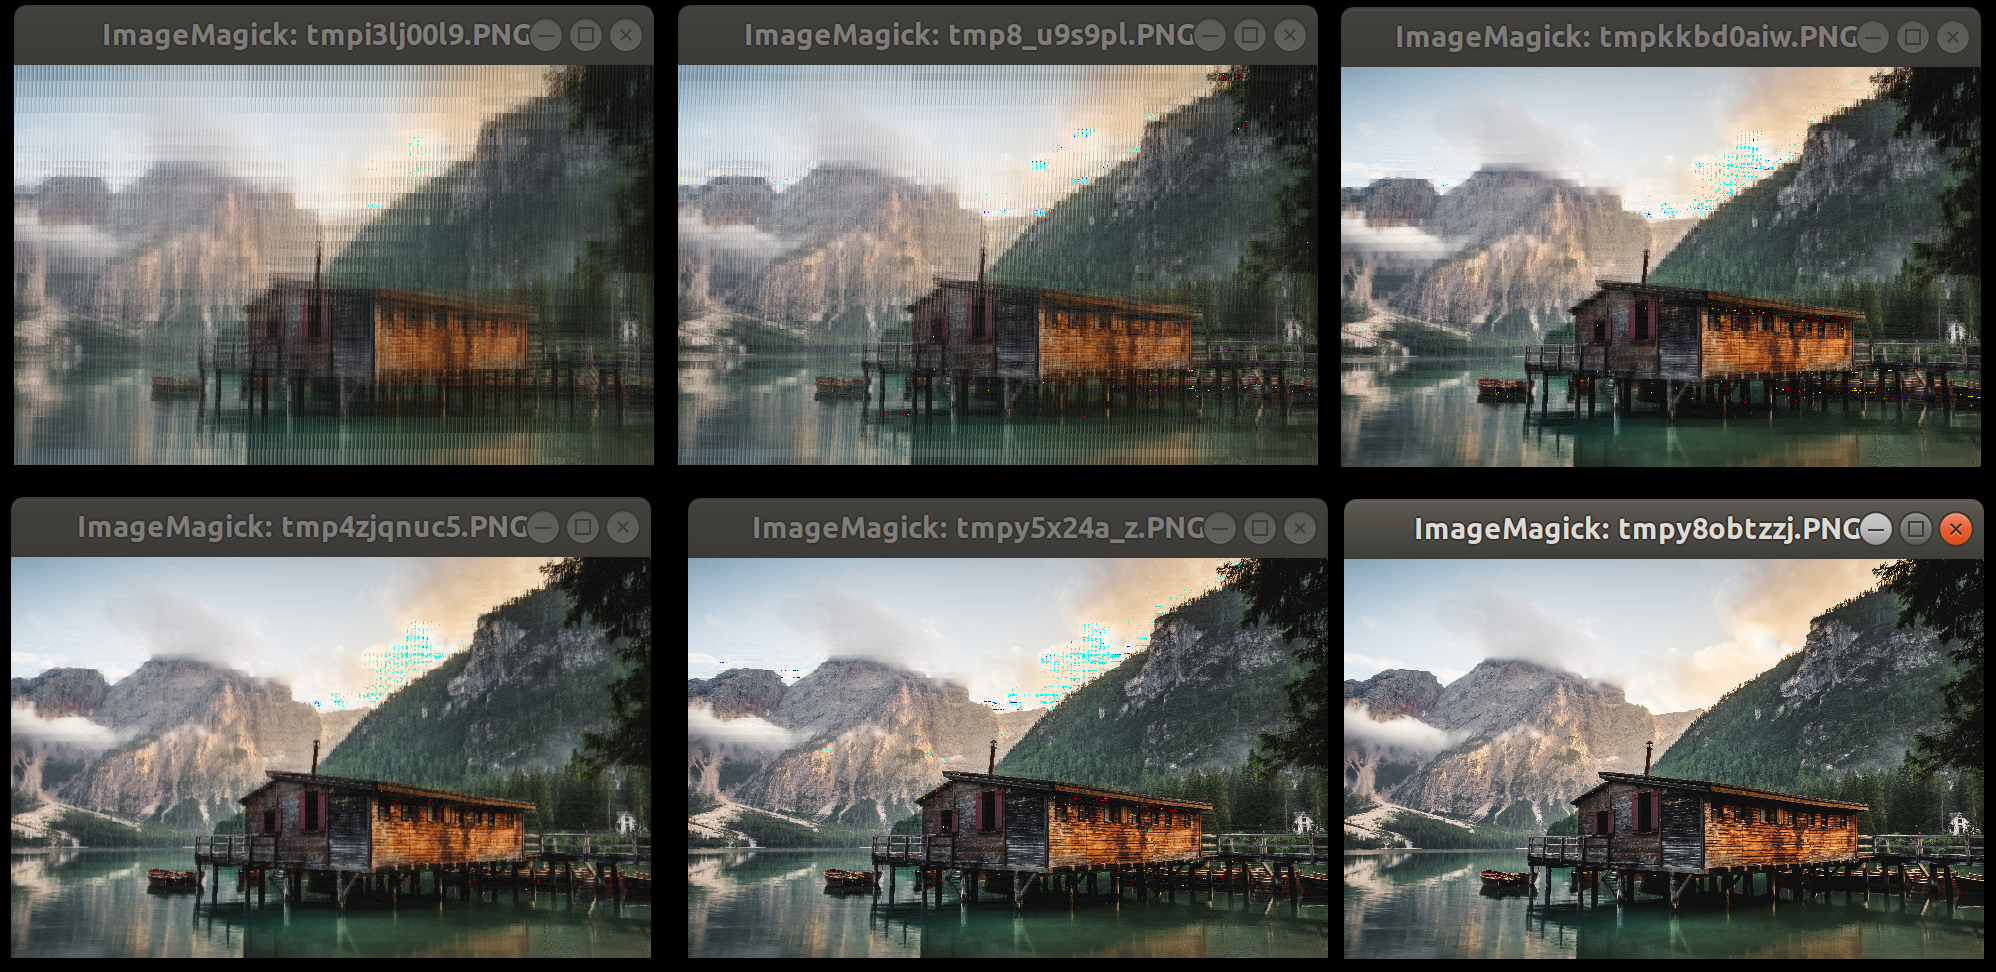
\includegraphics[width=\linewidth]{images/imgCompare2.png}
\subsection{Discussion}
